\section{Zadanie 3: Kwadratury Numeryczne}
\subsection{Charakterystyka Metody i problem} 
Numeryczne kwadratury stanowią metodę stosowaną do aproksymacyjnego obliczania całek oznaczonych poprzez odpowiednią sumę ważoną. Zadanie to sprowadza się do wyznaczenia wag \( Z_i \) oraz punktów \( L_i \), które spełniają określony warunek:
\[
\int_a^b f(x)dx \approx \sum_{i=1}^n f(L_i)Z_i,
\]
Przy czym punkty \( L_i \) są równomiernie rozmieszczone w przedziale \([a, b]\). Wyprowadzenie metody opiera się na założeniu, że skonstruowany system równań liniowych jest dokładny dla wielomianów określonego stopnia \( n-1 \). Dla uzyskania wyższej precyzji obliczeń, możliwe jest podzielenie przedziału \([a, b]\) na drobniejsze podprzedziały. Metody te są podstawą konstrukcji algorytmów rozwiązywania zagadnień 

\subsection{Metoda Rozwiązania} 
\begin{enumerate}

\item Chcemy rozwiązać problem postaci:
\[
    I(f) = \sum_{i = 0}^{n-1} Z_i \cdot f(L(i))  
\]
\item Formułowanie układu równań: Skonstrukowanie odpowiedniej macierzy oraz wektora wyrazów wolnych: \[
A_{ij} = L_j^i, \quad B_i = \frac{b^i - a^i}{i}.
\]
\item Rozwiązanie układu: Podejmujemy się rozwiązania układu równań liniowych \( AZ = B \), które charakteryzuje się: \[
\begin{bmatrix}
1 & 1 & \cdots & 1 \\
L_1 & L_2 & \cdots & L_n \\
L_1^2 & L_2^2 & \cdots & L_n^2 \\
\vdots & \vdots & \ddots & \vdots \\
L_1^{n-1} & L_2^{n-1} & \cdots & L_n^{n-1}
\end{bmatrix}
\begin{bmatrix}
Z_1 \\
Z_2 \\
\vdots \\
Z_n
\end{bmatrix} =
\begin{bmatrix}
b-a \\
\frac{b^2-a^2}{2} \\
\frac{b^3-a^3}{3} \\
\vdots \\
\frac{b^n-a^n}{n}
\end{bmatrix}.
\]\noindent 
\item Generowanie punktów interpolacji: Definiujemy punkty o równomiernym rozłożeniu jako: 
\[
L_i = a + i \frac{b-a}{n-1}, \quad i=0,1,\ldots,n-1.
\]
\end{enumerate}
\subsection{Przeprowadzone Testy} Przeprowadzono porównawcze testy różnych metod numerycznych stosowanych do obliczania całek: \begin{itemize}
    \item Riemannowskie sumy prostokątów.
    \item Klasyczne metody kwadratur (z równomiernymi punktami interpolacyjnymi).
    \item Kwadratury dzielone (podział przedziału na mniejsze części).
    \item Metoda \texttt{quad} z biblioteki \texttt{scipy}.
\end{itemize}
Testy przeprowadzono w przedziale \([2, 10]\), dla funkcji $\sin(x) + x^2, \ln(x)$: 
\begin{enumerate}
    \item Zmianę błędu całkowania w zależności od liczby punktów interpolacyjnych (od 2 do 100).
    \item Liczbę punktów potrzebnych do osiągnięcia określonej precyzji przy maksymalnej liczbie interpolacji $25 * (b-a)$. 
   \item Analiza zachowania zbieżności sumy w kontekście interpolowanego i całkowanego przypadku (gdzie wartość całki jest znana) w porównaniu do przybliżonego.
\end{enumerate}

\begin{minipage}{0.45\textwidth}
    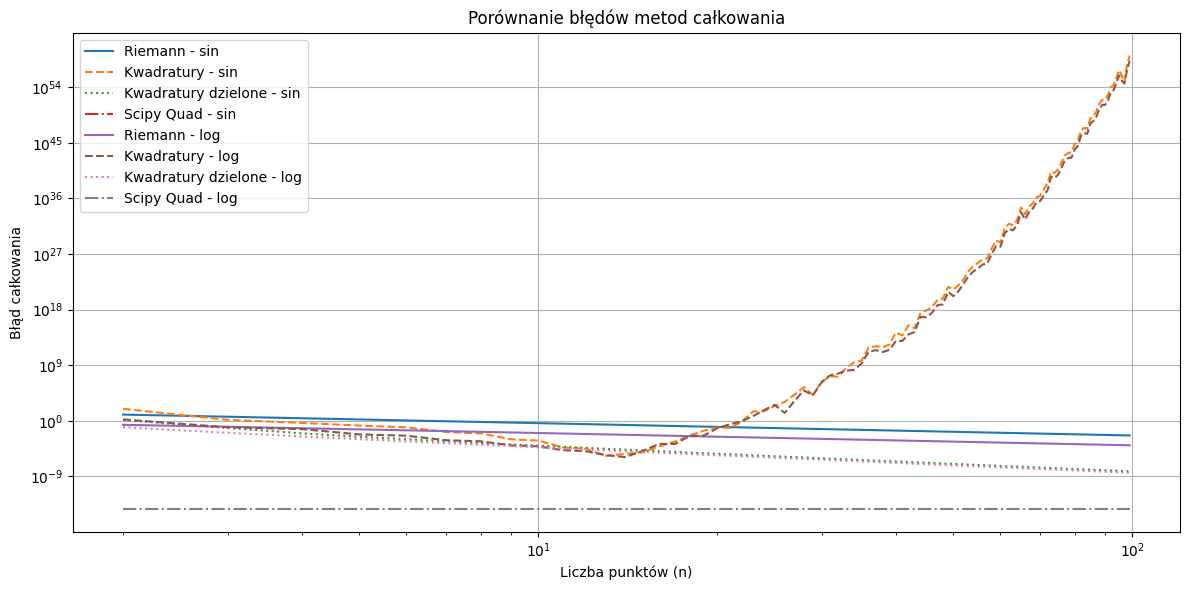
\includegraphics[width=\textwidth]{wykresy/zadanie 3/blad_punkty.png}
\end{minipage} 
\begin{minipage}{0.45\textwidth}
    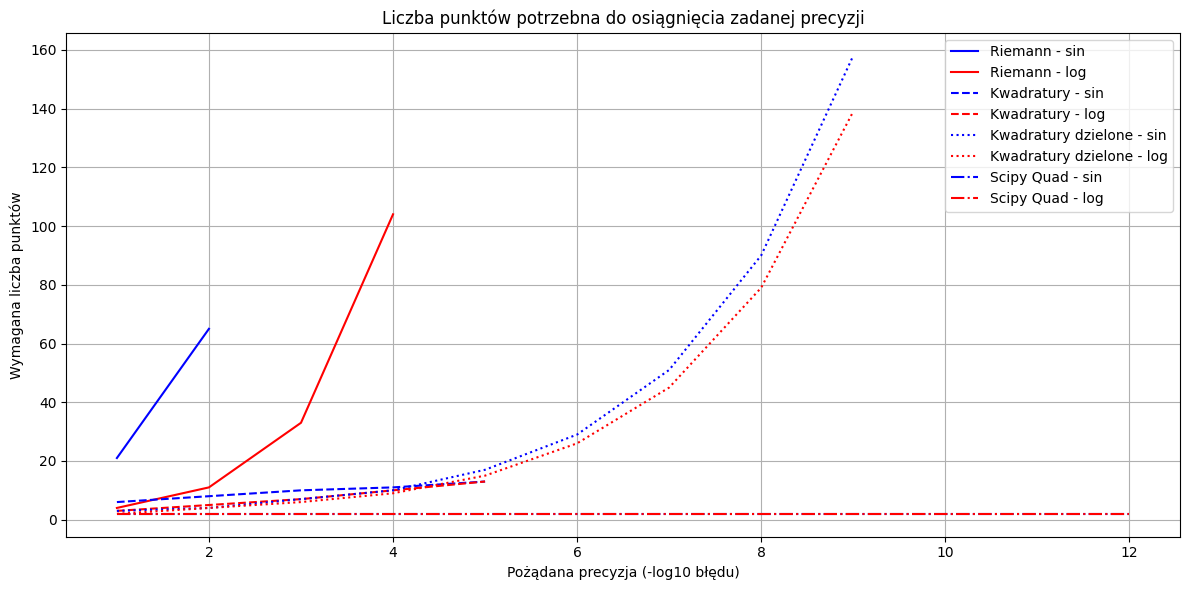
\includegraphics[width=\textwidth]{wykresy/zadanie 3/punkty_precyzja.png}
\end{minipage}

\begin{minipage}{0.92\textwidth}
    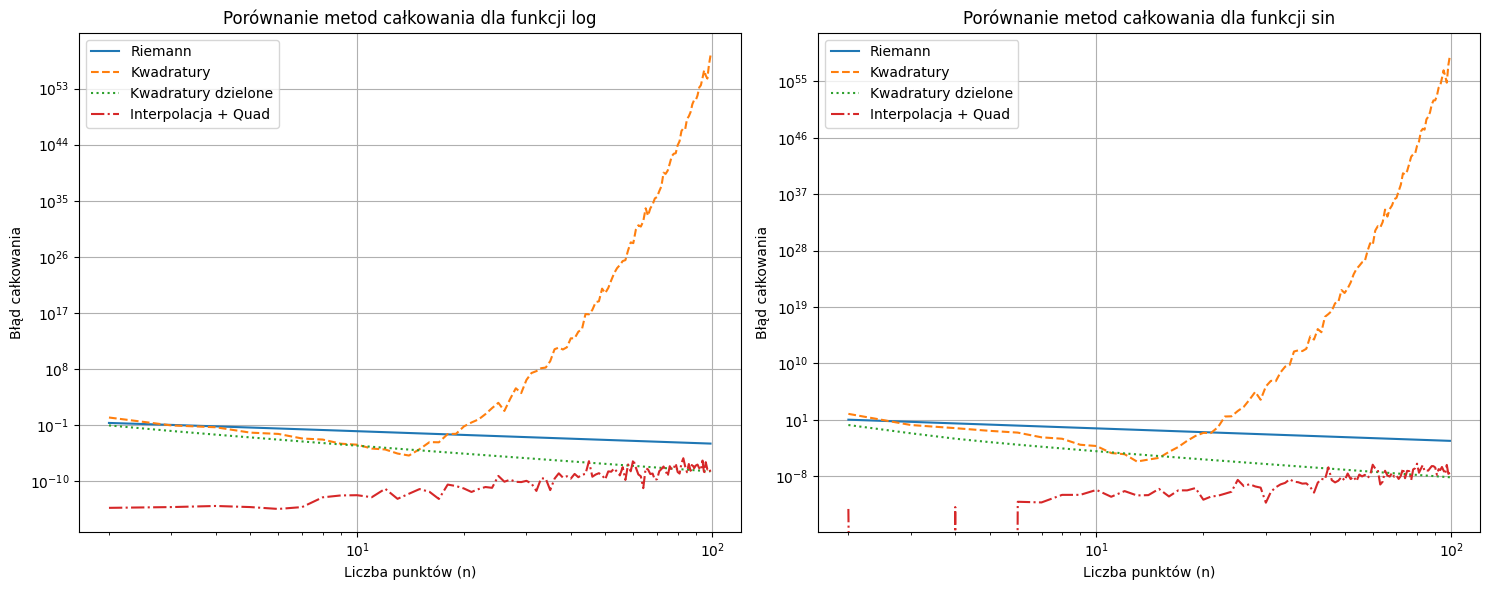
\includegraphics[width=\textwidth]{wykresy/zadanie 4/blad_punkty.png}
\end{minipage}

\subsection{Wnioski i analiza} 
\begin{itemize}
    \item Metoda sum Riemanna jest najmniej efektywna i nawet przy bardzo dużej liczby punktów nie jest w stanie osiągnąć szukanej prezycji.
    \item Widać że zwykłe kwadratury nie są tak efektywne, jak dzielone. Wypadają one także znacznie gorzej obliczeniowo, ponieważ najbardziej złożonym prosem jest rozwiązanie macierzy. 
    \item Kwadratury dzielone oferują znaczną poprawę dokładności, jednak są wolniejsze i mniej dokładne od wbudowanej funkcji \texttt{quad}.
    \item Metoda \texttt{quad} osiąga najlepsze wyniki dzięki nierównomiernemu doborowi punktów interpolacyjnych oraz wykorzystaniu wielomianów Legendre’a, co pozwala na precyzyjną aproksymację trudnych funkcji. % TODO odnośnik zamieścić
    \item Widzimy że metoda polegająca na wcześniejszym liczeniu wielomianu interpolowanego jest korzystniejsza. Błąd zależy wtedy tylko i wyłącznie od przyblizenia %TODO odnieść się do artykułu (AGH)
\end{itemize}
\paragraph{Złożoność obliczeniowa}:
\begin{itemize}
    \item Riemannowskie sumy prostokątów: \( O(n) \).
    \item Klasyczne kwadratury: \( O(n^3) \) (rozwiązanie układu równań).
    \begin{itemize}
        \item stworzenie macierzy $O(n^2)$
        \item Rozwiązanie układyu równań $O(n^3)$ - metoda $LU$ %TODO odnośnik do strony z dokumentacją
        \item Zatem złożoność $O(n^3)$
    \end{itemize}
    \item Kwadratury dzielone: \( O(k \cdot n^3) \), gdzie \( k \) to liczba podprzedziałów, \( n \) oznacza ilość punktów w podprzedziale u nas \(n=3\).
    \item \texttt{quad}: Adaptacyjna metoda z nierównomiernym wyborem punktów, której złożoność zależy od funkcji, ale w praktyce jest bardzo efektywna, dzięki zastosowaniu wielomianów Legendre'a. %TODO to bibliografii się odnieść 
\end{itemize}

% O ile rośnie dokładnośc z każdą iteracją ~ to jest charakterystyka do znalezienia !!!!

% TODO 
% dodać bilbiografie, ref'y zrobić 
% trochę ten tekst zredagować żeby to lepiej wyglądało
% poszukać książek gdzie to opisują i się do tego jakoś odnieść